% Created 2022-10-16 Sun 21:58
% Intended LaTeX compiler: pdflatex
\documentclass[11pt]{article}
\usepackage[utf8]{inputenc}
\usepackage[T1]{fontenc}
\usepackage{graphicx}
\usepackage{longtable}
\usepackage{wrapfig}
\usepackage{indentfirst}
\usepackage{rotating}
\usepackage[normalem]{ulem}
\usepackage{amsmath}
\usepackage{amssymb}
\usepackage{capt-of}
\usepackage{hyperref}
\usepackage[dvipsnames]{xcolor}
\usepackage{tikz}
\usetikzlibrary{shapes,arrows,positioning,calc}
\usepackage{listings}
\usepackage{color}
\usepackage[utf8]{inputenc}
\usepackage{mathtools}
\usepackage{amsmath}
\usepackage{amsfonts}
\usepackage[margin=1.0in]{geometry}
\usepackage{mdframed}
\BeforeBeginEnvironment{minted}{\begin{mdframed}}
\AfterEndEnvironment{minted}{\end{mdframed}}
\date{\today}
\title{}
\hypersetup{
 pdfauthor={Ben Anderson},
 pdftitle={UR3e Documentation},
 pdfkeywords={},
 pdfsubject={},
 pdflang={English}}
\begin{document}

\tikzset{
block/.style = {draw, fill=white, rectangle, minimum height=3em, minimum width=3em},
tmp/.style  = {coordinate}, 
sum/.style= {draw, fill=white, circle, node distance=1cm},
input/.style = {coordinate},
output/.style= {coordinate},
pinstyle/.style = {pin edge={to-,thin,black}
}
}

\newcommand\connect[2]{\path[draw,arrow] (#1) |- ($(#1)!1/2!(#2)$) -| (#2)}

% \setcounter{secnumdepth}{0}
\author{Ben Anderson}
% \date{\today}
\title{UR3e OCE Stabilization System}
\maketitle
\tableofcontents
\parskip=6pt

\section{Planning (Delete later)}
Introduction section will summarize the body of the text,

I need a section detailing the interfaces of the UR3e robot and why I need to use the workaround that I have

I need a section detailing how my code works to optimize the strength of the input signal

I need a section detailing how all of these bits of code interact with each other (will be the hard bit)

Creative decision: I could either lead with the section detailing how all the components interact with each other, or I could lead with sections detailing individual components and close with a section summarizing their overlap. The tradeoff is the summary section will be missing a lot of context, but this could potentially be provided by linking forwards repeatedly. Mayhaps this is the move. I just need to learn how to link to a place further along in a document (\autoref{sec:hello}).

Okay that looks promising to me. Lets go with that.

\section{Introduction}\label{sec:hello}

The focus of my work for the better part of the last year has been studying how to use a UR3e Cobot for the purposes of focusing and stabilizing a sensor at its focal length away from a target surface. This has involved a thorough examination of the API and programming tools that accompany the Universal Robots ecosystem, as well as creating systems for synchronizing the robotic control system with signal processing and sensor systems.

In doing so a number of systems are being used in ways for which they were not designed. The consequence of this is that my codebase resembles a kludgy pile of half-fixes and temporary-solutions that, technically, have achieved the objective, at the expense of stability and ease of use.
In recent months more efforts have been made to improve the readability of the codebase and allow for easier changes later on, but the work is ongoing and the project cannot wait for me to complete this work.

The hope is with this documentation, others in the OCE project can gain enough of an understanding of how the system works to use it in my absence as well as modify or extend the platform I've built.

Due to the kludgy nature of the platform, it may not be suitable to read this guide linearly. The introduction section should hopefully give you an overview of how the components of this section communicate and interface with each other, and a more thorough description of the workings of each module are in the following chapters.\\
If you are planning to operate the robot I would recommend reviewing the section on operating the robot through the control pendant (\autoref{sec:pendant}) and the section on running the code (\autoref{sec:startup}).

\section{Overview of Transudcer Alignment system}
\begin{center}
\begin{tikzpicture}[auto, node distance=3cm, on grid,auto,>=latex']
\node[block] (sensor) {Sensor};
\node[block, right = of sensor] (robot) {UR3e};
\node[block, right = of robot] (URScript) {URScript};
\node[block, below = of sensor, align=center] (labview) {Signal\\Processing};
\node[block, right = of labview, align=center] (socket) {Internal\\Socket Server};
\node[block, right = of socket, align=center] (tcc) {Control\\Code};

\draw [draw, <-] (robot) -- (URScript);
\draw [->] (sensor) -- (robot);
\draw [draw, <->] (sensor) -- (labview);
\draw [->] (labview) -- (socket);
\draw [<->] (socket) -- (tcc);
\draw [<->] (socket) |- ($(socket)!1/2!(socket |- URScript)$) coordinate (C) -| (URScript);

\node[text=black, below left= 6mm and 12mm of tcc.west] (pc) {PC};
\draw[black, dashed] (pc.east)-|([xshift=3mm]tcc.east)|-([yshift=3mm]socket.north)-|([xshift=-4mm]labview.west)|-(pc.west);

\node[text=black, above right= 6mm and 4mm of robot.east] (ur) {STANLEy};
\draw[black, dashed] (ur.east)-|([xshift=3mm]URScript.east)|-([yshift=-3mm]robot.south)-|([xshift=-4mm]robot.west)|-(ur.west);

\end{tikzpicture}
\end{center}

The sensor is a generic device that requires focusing and produces an output that is read by the signal processing package within the computer. The Stabilization and Transducer Alignment for Nearby Laser Elastography system (hencforth referred to as STANLEy) consists of a UR3e cobot from Unviersal Robots, and a script written in using the Universal Robots proprietary scripting language. \\
(Attempts are being made to reverse-engineer some of this languages functions to cut this box out of the control diagram, but the process will be very involved and is being put off in order to meet deadlines).

Physically, this system includes a robotic arm manipulator, a control box, and a teaching pendant.
STANLEy interfaces with the sensor through a physical linkage at the end of the robotic manipulator, and with the PC through an ethernet cable.

The remaining control blocks occur within a nearby computer. The signal processing block refers to a program (typically in MATLAB or LabView) which recieves the data from the sensor and processes it for further use. 
\emph{For the purposes of the control loop that focuses the sensor, the signal processing block must reduce the sensor input, no matter how complex, to a simple magnitude that should be maximized to bring the sensor into alignment.}\\
An internal socket server is spun up in a simple python program. This is a program that listens on a hard-coded IP-address and port within the computer for input sent from the signal processing block, the control code, and to the robot through the control box. More on the limitations of this system in the section on running the code (\autoref{sec:startup})\\
The control code is run from a script named \texttt{TransducerHoming.py}, and associated libraries. For now, directly editing this file is the main interface with which we can modify how the homing sequence runs.
In future I hope to expand the user interface as well as the command-line options to allow more on-the-fly modification of program parameters, but the duration off tests and the speed at which changes are made have made this an inefficient goal for some time.

Overall the system utilizes three discrete devices and at least three programming languages. I (Ben Anderson) am most directly involved with the programming of the control code and URScript. The top-down overview of each components' functions are pretty simple, but debugging/modifying them will require a rough understanding of the URScript API and a strong understanding of Python.

\section{STANELEy and the URScript API}\label{sec:robot_summary}

The body of the novelty surrounding this project centers around the use of a UR3e robotic arm to position and hold the OCE sensor. \\
The UR3e is manufactured by Universal Robots and is primarily designed to automate human labor. Shipped with the robotic arm is a control box and a teach pendant, a hand-held tablet for manually controlling the robot. The control box allows one to write and execute scripts using the proprietary URScript API, a set of functions built into the robot that handle common tasks related to positioning and animating the arm.
Additionally, the control box has an ethernet port supporting the secondary and Real Time Data Exchange interfaces. Both of these have their uses and can be read about in the \hyperlink{https://www.universal-robots.com/articles/ur/interface-communication/remote-control-via-tcpip/}{remote control interface guide}, however they weren't adequate for the method ultimately used. \\




\subsection{The Teach Pendant and the PolyScope interface}\label{sec:pendant}
The teach pendant is the default accesory for interacting with the internals of the robot. It is shipped with the robot along with the control box.
\begin{center}
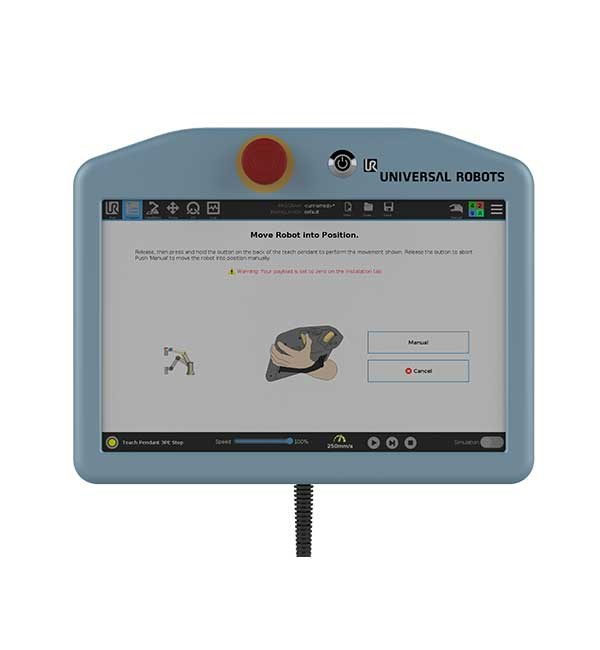
\includegraphics[width=.8\linewidth]{figures/teach_pendant.jpg}
\end{center}
The pendant, when active, is running an interface known as PolyScope, the GUI used for operation of all UR robots. Along the top of the page, there are six different menus and a file explorer interface that we will refer to later:

\begin{center}
\includegraphics*[width=.9\linewidth]{figures/menu_banner.jpg}
\end{center}

The full manual for PolyScope can be read \hyperlink{https://s3-eu-west-1.amazonaws.com/ur-support-site/114079/99403_UR3e_User_Manual_en_Global.pdf\#page=107\&zoom=100,76,233}{here}, but this guide will cover the elements necessary for operation of STANLEy.

\subsubsection{Initialization and setup}
In order to use the robot, power on the tool box by pressing the physical power button above the screen and next to the e-stop on the teach pendant. 
(It can be finicky how long a press is necessary, so if you suspect you're holding the button down too long listen for a click from the control box to indicate it has been powered on. You should release the button immediately after hearing this click).\\
The power button should light up green and the screen should show a loading screen as the robot takes a minute to boot up.\\

Upon fully booting up, the robot itself still remains dormant. In the bottom-left of the screen is the \uline{robot status indicator}, shown here:

\begin{center}
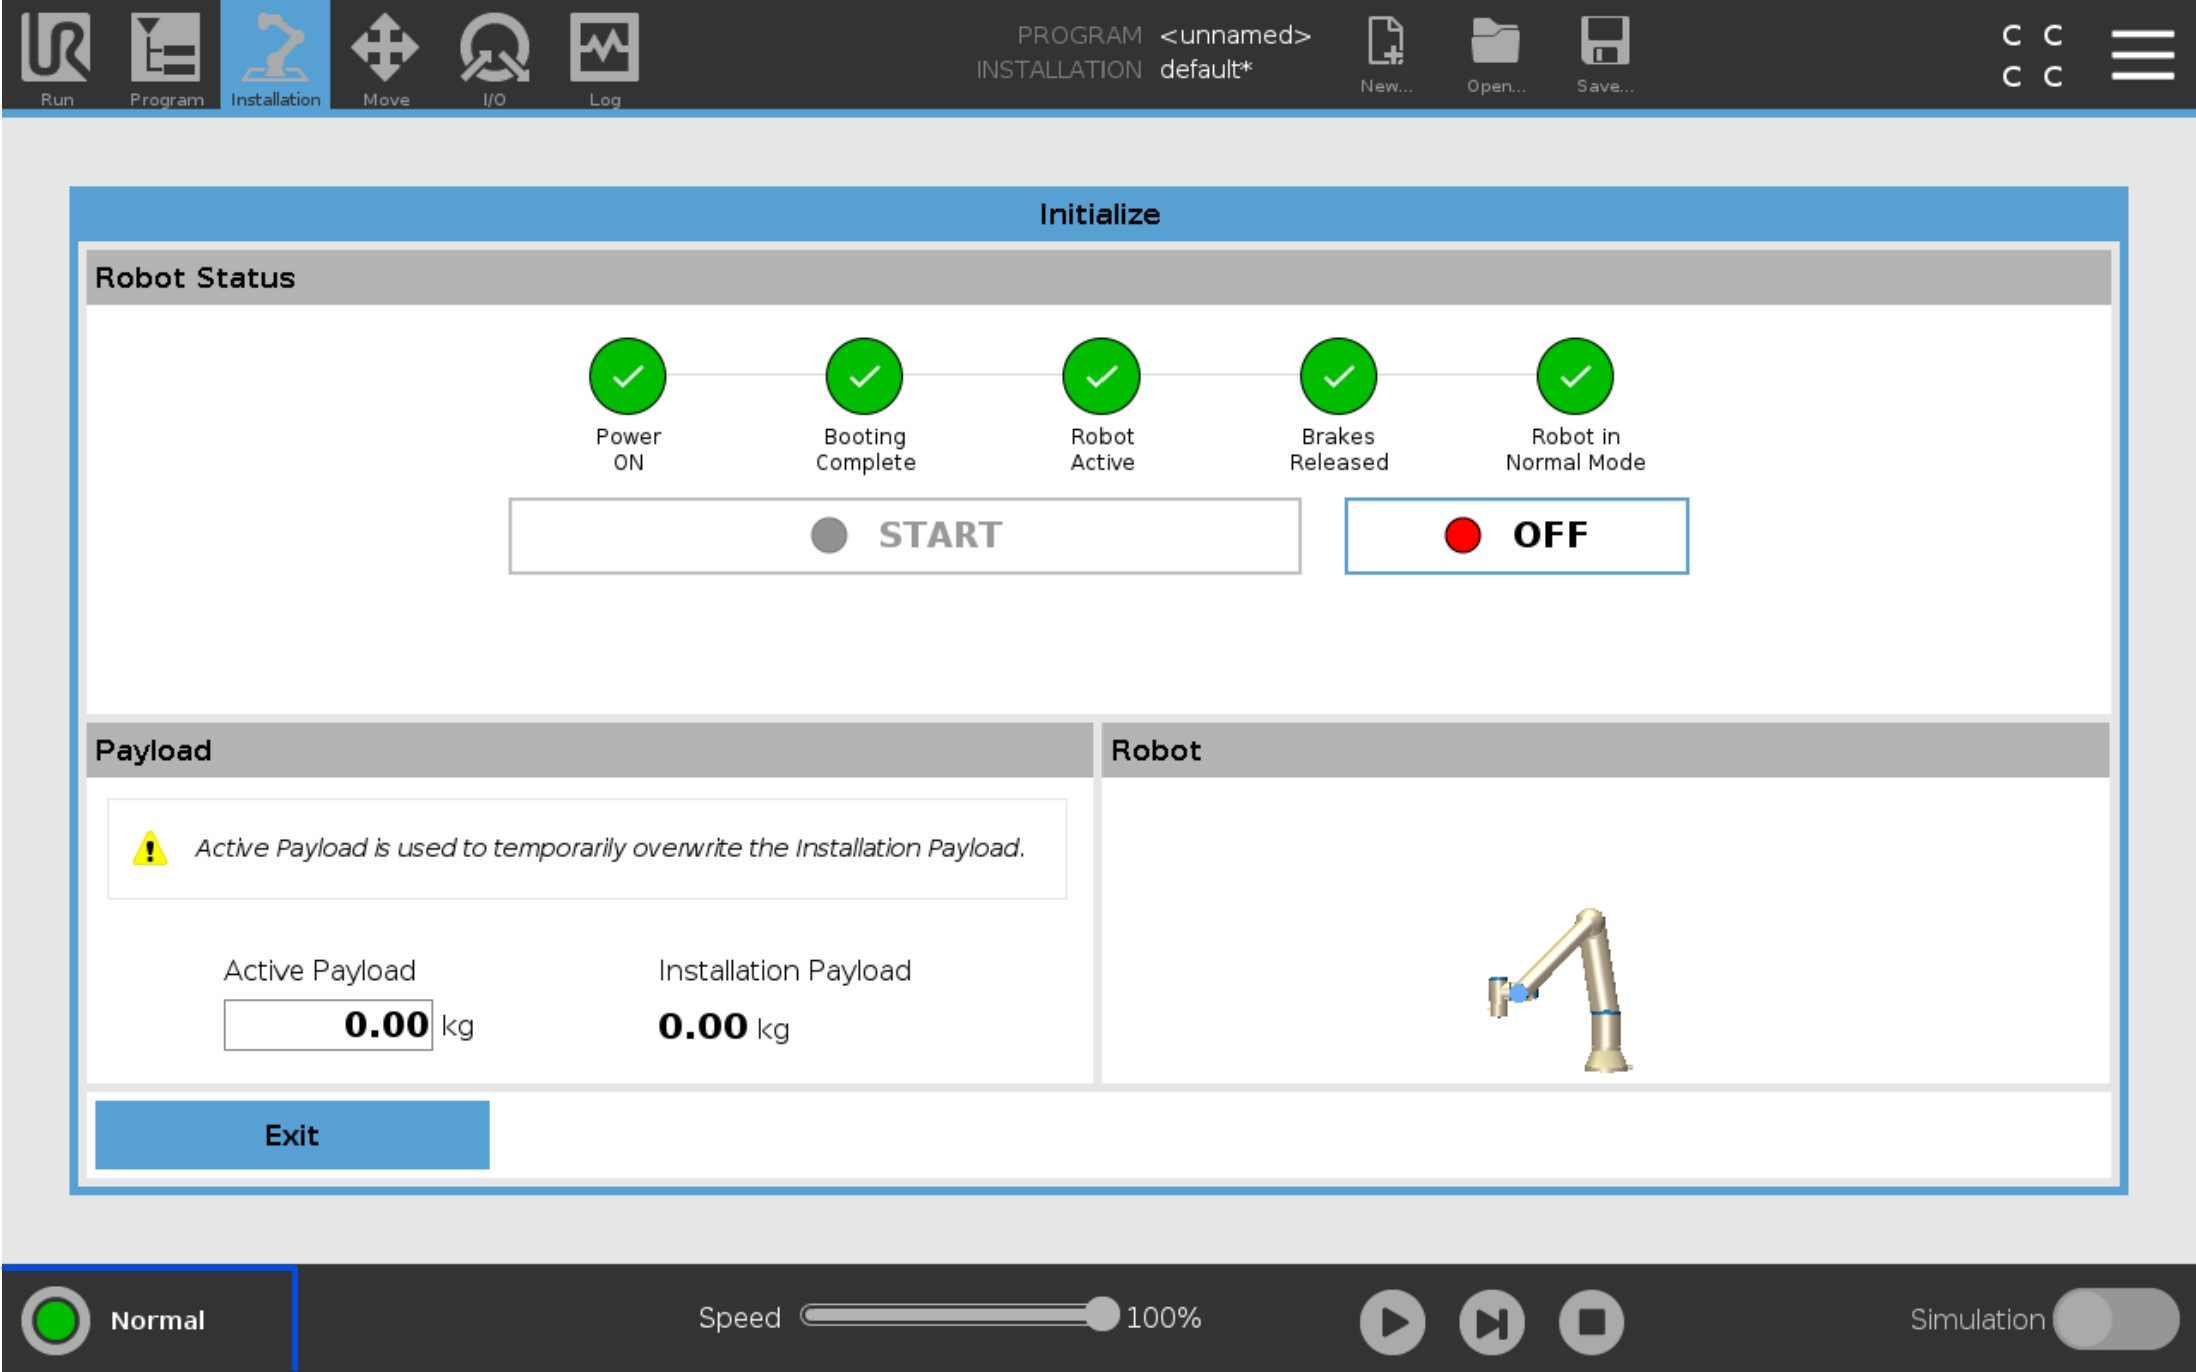
\includegraphics[width=.9\linewidth]{figures/robot_state_menu.jpg}
The color inside the circle indicates the state of the robot:
\end{center}
\begin{itemize}
    \item \emph{Red}: The robot is powered off.
    \item \emph{Blue}: The robot is in freedrive mode.
    \item \emph{Yellow}: The robot is idle; powered on but not ready for operation.
    \item \emph{Green}: Powered on and ready for normal operation.
\end{itemize}

After booting up the control box you enter the Initialization screen (shown in the image above). When powering up the robot from full-shutdown the central button will be active and you will press it twice to enable the robot; first it will say `ON` and you press it to deliver power to the robot, then it will say `START` and you will press it to unlock the brakes and enable the robot completely.\\

\emph{Warning:} The robot will move slightly as the brakes are unlocked, do not leave the robot in a stat where this motion will put nearby equipment at risk.

\subsubsection*{Program tab}
The program tab is one of the options in the menu tab. Here is where you write/modify URScript programs. The UR3e used in our lab has a program saved already that can be opened by tapping the "open" button in the top banner and tapping "Program" from the subsequent dropdown. (The program written for this lab is still called \texttt{test.urp})

\subsection{URScript API}\label{sec:urscript}

\section{Python + the control loop}\label{sec:control_code}
\subsection{Startup guide}\label{sec:startup}
There isn't really content here yet.
\subsection{TransducerHoming.py}\label{sec:TransducerHoming}

STANLEy -> Stabilization and Transducer Alignment for Nearby Laser Elastography
\begin{center}
    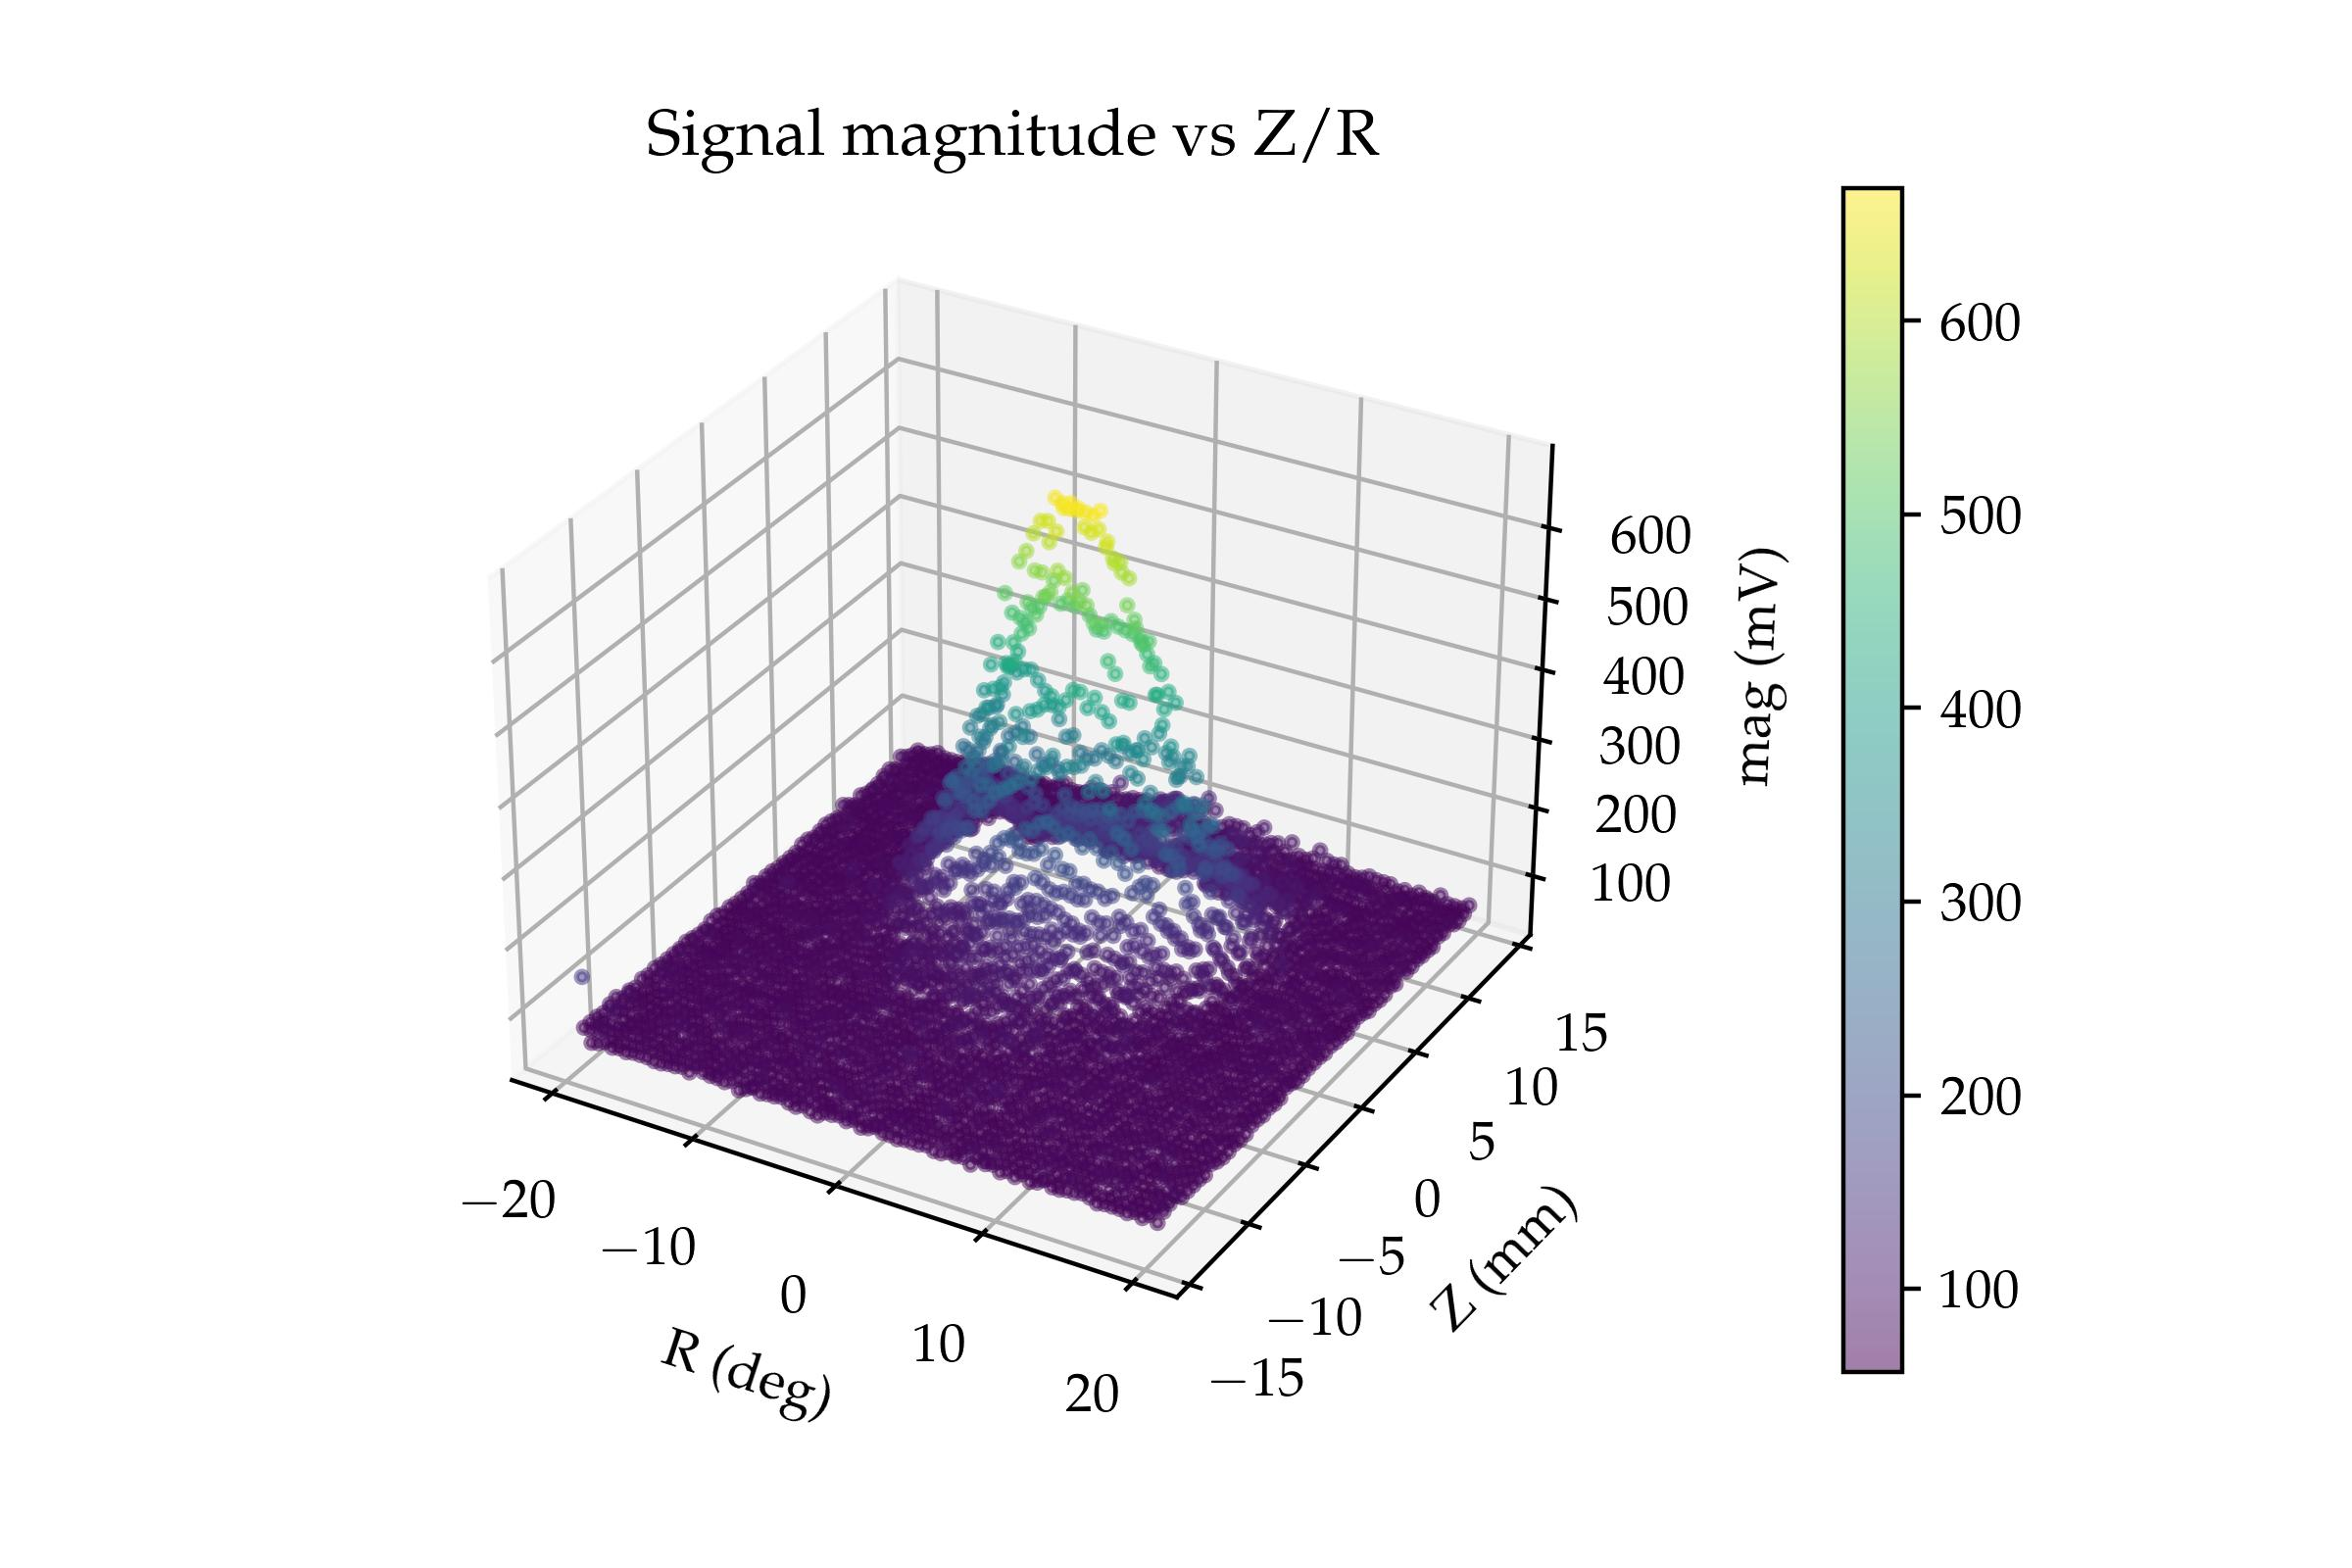
\includegraphics[width=.9\linewidth]{../Debugging Scripts/figures/2D_fullscan_render_test_10.jpg}
\end{center}

\begin{center}
    \includegraphics[width=.9\linewidth]{c:/Users/ander/Sync/Screenshots/22_10_18_4.png}
\end{center}


\end{document}